%%%%%%%%%%%%%%%%%%%%%%%%%%%%%%%%%%%%%%%%%%%%%%%%%%%%%%%%%%%%%%%%%%%%%%%%%%%%%%%%
% SmartIrrigate Home - Business Plan
% Autori: Federico Dellini, Danilo Amalfitano (CEO, SmartIrrigate)
% Data: 1 Giugno 2026
%%%%%%%%%%%%%%%%%%%%%%%%%%%%%%%%%%%%%%%%%%%%%%%%%%%%%%%%%%%%%%%%%%%%%%%%%%%%%%%

\documentclass[11pt,a4paper]{report}
\usepackage[utf8]{inputenc}
\usepackage[T1]{fontenc}
% Use English babel if Italian support is not available on the system
\usepackage[english]{babel}
\usepackage{geometry}
\geometry{left=2.5cm,right=2.5cm,top=2.5cm,bottom=2.5cm,headheight=14pt,headsep=25pt}
\usepackage{graphicx}
\usepackage{float}
\usepackage{booktabs}
\usepackage{multirow}
\usepackage{array}
\usepackage{longtable}
\usepackage{hyperref}
\hypersetup{
    colorlinks=true,
    linkcolor=blue,
    urlcolor=blue,
    citecolor=black,
    pdfencoding=auto
}
\usepackage{parskip}
\setlength{\parskip}{0.8em}
\usepackage{enumitem}
\setlist[itemize]{noitemsep,topsep=0pt,parsep=0pt,partopsep=0pt,leftmargin=*}
\setlist[enumerate]{noitemsep,topsep=0pt,parsep=0pt,partopsep=0pt,leftmargin=*}

%===== COLORS =====
\usepackage{xcolor}
\definecolor{warningcolor}{HTML}{FF6B6B}
\definecolor{successcolor}{HTML}{51CF66}
\definecolor{infocolor}{HTML}{4C6EF5}

%===== INTESTAZIONI =====
\usepackage{fancyhdr}
\pagestyle{fancy}
\fancyhf{}
\rhead{\thepage}
\lhead{SmartIrrigate Home - Business Plan}
\rfoot{}
\lfoot{}

%===== STILI SEZIONI =====
\usepackage{sectsty}
\chapterfont{\fontsize{14pt}{16pt}\selectfont\bfseries\centering}
\sectionfont{\fontsize{12pt}{14pt}\selectfont\bfseries}
\subsectionfont{\fontsize{11pt}{13pt}\selectfont\bfseries\itshape}

%===== SIMBOLI PER SOSTITUIRE UNICODE =====
\usepackage{amssymb}
\usepackage{amsmath}
\usepackage{tikz}
\usepackage{textcomp}
\usepackage{eurosym}
\newcommand{\checkmarkbold}{\textbf{\checkmark}}
\newcommand{\crossbold}{\textbf{\texttimes}}
\newcommand{\textwarning}{\textcolor{warningcolor}{$\blacktriangle$}}

%===== ALLINEAMENTO TABELLE =====
\newcolumntype{L}[1]{>{\raggedright\arraybackslash}p{#1}}
\newcolumntype{C}[1]{>{\centering\arraybackslash}p{#1}}

\begin{document}

%===== COPERTINA =====
\title{
     \begin{figure}[H]
         \centering
         \IfFileExists{Image/Logo_SmartIrrigate_Home_v2.png}{%
            \includegraphics[width=0.5\linewidth]{Image/Logo_SmartIrrigate_Home_v2.png}%
         }{}
     \end{figure}
    \textbf{SmartIrrigate Home} \\ \Large Business Plan
}
\author{Federico Dellini (CEO, SmartIrrigate) \\ Danilo Amalfitano (CTO, SmartIrrigate)}
\date{1 Giugno 2026}

\maketitle
\thispagestyle{empty}
\newpage

\tableofcontents
\thispagestyle{empty}
\newpage

\chapter{SINTESI ESECUTIVA}

\section{Opportunità di Mercato}
SmartIrrigate Home opera nel mercato italiano dell'irrigazione intelligente per balconi, terrazze e giardini urbani. Il Mercato Totale Indirizzabile (TAM) è di \textbf{€400-500M/anno} per i sistemi di irrigazione domestici, con un Mercato Disponibile Servibile (SAM) di \textbf{€40-50M/anno} per le soluzioni intelligenti. Il mercato dimostra un forte potenziale di crescita con un CAGR del \textbf{11-12\%} previsto dal 2020 al 2026.

\section{Servizi}
Il nostro prodotto combina la tecnologia IoT all'avanguardia con la precisione agronomica:
\begin{itemize}
    \item \textbf{Raccolta di Energia}: Sistema alimentato a energia solare con 5-7 anni di autonomia (vs. 6-12 mesi per i concorrenti)
    \item \textbf{Algoritmo Predittivo}: Calcolo ET\textsubscript{0} + Kc integrato con previsioni meteorologiche a 48 ore
    \item \textbf{Irrigazione Selettiva}: Controllo a livello di singola pianta tramite valvole PWM bistabili
    \item \textbf{Installazione Plug \& Play}: Configurazione completa in meno di 1 ora
\end{itemize}

\section{Strategie di Marketing e Vendita}
\textbf{Proposta di Vendita Unica (USP)}: SmartIrrigate Home è l'unico sistema di irrigazione intelligente con 5-7 anni di autonomia energetica, algoritmo predittivo ET\textsubscript{0}+Kc e irrigazione personalizzata per ogni pianta.

\textbf{Segmenti di Mercato di Riferimento}:

\begin{longtable}{|p{3cm}|p{2.5cm}|p{3cm}|p{4cm}|}
\hline
\textbf{Segmento} & \textbf{Budget (€)} & \textbf{Canale Primario} & \textbf{Problema} \\ \hline
Giovane Giardiniere Urbano & 150-250 & E-commerce (65\%) & Dimenticanza - le piante muoiono durante i viaggi \\ \hline
Pensionato con Orto & 100-200 & Negozi fisici (35\%) & Fatica fisica, artrite \\ \hline
Condominio Eco-Sostenibile & 500-2.000 & Gare B2B & Spreco d'acqua nei sistemi centralizzati \\ \hline
\end{longtable}

\section{Dati Finanziari Principali}
\textbf{Indicatori Chiave di Prestazione}:
\begin{itemize}
    \item \textbf{CAC}: €80-100 (obiettivo: €80)
    \item \textbf{LTV}: €300-400 (obiettivo: €350 con abbonamento SaaS)
    \item \textbf{Rapporto LTV:CAC}: 3,5-5:1 (standard di eccellenza >3:1)
    \item \textbf{Margine Lordo}: 45-50\%
    \item \textbf{Punto di Pareggio}: 10.560 unità/anno (€2,40M di ricavi/anno)
\end{itemize}

\textbf{Proiezioni dei Ricavi}:

\begin{longtable}{|p{1.5cm}|p{2cm}|p{2cm}|p{1.5cm}|p{1.5cm}|p{2cm}|}
\hline
\textbf{Anno} & \textbf{Unità Vendute} & \textbf{Ricavi (€M)} & \textbf{CAC (€)} & \textbf{LTV (€)} & \textbf{Margine Lordo} \\ \hline
2026 & 5.000 & 0,75-1,25 & 100 & 300 & 45\% \\ \hline
2027 & 15.000 & 2,25-3,75 & 80 & 350 & 48\% \\ \hline
2028 & 30.000 & 5,0-8,0 & 70 & 400 & 50\% \\ \hline
\end{longtable}

\chapter{PANORAMICA AZIENDALE}

\section{Struttura di Proprietà}
SmartIrrigate Home è strutturata come una società a responsabilità limitata (S.r.l.) con la seguente distribuzione della proprietà:
\begin{itemize}
    \item \textbf{Fondatori}: 60\% (John Doe - AD, Jane Doe - Direttore Operativo)
    \item \textbf{Investitori Angel}: 30\%
    \item \textbf{Stock Options per Dipendenti}: 10\%
\end{itemize}

\section{Dichiarazione di Missione}
Rivoluzionare il giardinaggio urbano in Italia combinando l'innovazione tecnologica con la sostenibilità ambientale, rendendo l'irrigazione intelligente accessibile, conveniente e senza sforzo per ogni famiglia.

\section{Storia Aziendale}
Fondata all'inizio del 2026, SmartIrrigate è nata da un team di ingegneri IoT, agronomi e imprenditori che hanno identificato una lacuna critica nel mercato italiano: i sistemi di irrigazione intelligente esistenti o mancavano di una vera autonomia energetica o non fornivano precisione a livello di singola pianta. La visione fondante dell'azienda era creare un sistema che elimini i cicli di sostituzione delle batterie fornendo al contempo un'intelligenza di irrigazione di livello professionale agli utenti residenziali.

\section{Obiettivi Futuri}
\textbf{Breve termine (2026)}: Lancio del MVP con 5.000 unità vendute, ottenere un punteggio NPS >50, ridurre il CAC da €100 a €80 attraverso programmi di referenza e partenariati con influencer.

\textbf{Medio termine (2027-2028)}: Raggiungere il punto di pareggio, espandersi nei mercati francese e spagnolo, lanciare l'abbonamento SaaS SmartIrrigate a €4,99/mese per analisi avanzate e archiviazione storica dei dati.

\textbf{Lungo termine (2029+)}: Ottenere una quota di mercato del 5\% nel SAM italiano (€2M-2,5M di ricavi), introdurre SmartIrrigate Pro per l'agricoltura commerciale, perseguire la certificazione ISO 9001 e il riconoscimento del marchio ecologico dell'UE.

\chapter{ANALISI DI MERCATO}

\section{Mercato di Riferimento}
Il mercato italiano dell'irrigazione intelligente serve tre segmenti principali con caratteristiche distinte:

\textbf{Giovane Giardiniere Urbano (60\% delle vendite)}
\begin{itemize}
    \item Età: 25-35 anni
    \item Reddito: €25.000-40.000 annui
    \item Località: Grandi città (Milano, Roma, Torino)
    \item Piante: 5-10 piante ornamentali/aromatiche sui balconi
    \item Comportamento d'acquisto: Online-first, influenzato dai social media e dalle recensioni tecnologiche
\end{itemize}

\textbf{Pensionato con Orto (20\% delle vendite)}
\begin{itemize}
    \item Età: 60-75 anni
    \item Reddito: €20.000-30.000 (pensione)
    \item Località: Periferie e centri urbani più piccoli
    \item Piante: Orto sul terrazzo (10-20 m\textsuperscript{2})
    \item Comportamento d'acquisto: Preferisce i negozi fisici, apprezza semplicità e affidabilità
\end{itemize}

\textbf{Condominio Eco-Sostenibile (20\% delle vendite)}
\begin{itemize}
    \item Età: 35-50 anni
    \item Reddito: €40.000-60.000 annui
    \item Località: Condomini urbani con spazi verdi condivisi
    \item Piante: Aree comuni (50-200 m\textsuperscript{2})
    \item Comportamento d'acquisto: Gare B2B, valuta sostenibilità e ROI collettivo
\end{itemize}

\section{Dimensione del Mercato e Potenziale di Crescita}

\textbf{Segmentazione del Mercato}:

\begin{longtable}{|p{3cm}|p{3cm}|p{3cm}|p{2.5cm}|}
\hline
\textbf{Segmento} & \textbf{Target di Popolazione} & \textbf{Penetrazione Irrigazione} & \textbf{Valore TAM (€/anno)} \\ \hline
Famiglie con balconi/terrazze & ~13,5M famiglie & 8\% & €680M \\ \hline
Giardini urbani & ~24M coltivatori & 5\% & €420M \\ \hline
Condomini con aree verdi & ~4,2M condomini & 12\% & €750M \\ \hline
\end{longtable}

\textbf{Motori di Crescita}:
\begin{itemize}
    \item \textbf{Espansione del Mercato Smart Home}: +11\% di crescita in Italia, mercato superato €1B nel 2025
    \item \textbf{Boom del Giardinaggio Urbano}: +18,5\% di aumento dal 2020 (dati Coldiretti)
    \item \textbf{Sensibilizzazione Ambientale}: 77\% degli europei sceglie la tecnologia smart per il giardinaggio
    \item \textbf{Preoccupazioni per la Scarsità d'Acqua}: 62\% degli italiani si preoccupa delle condizioni di siccità estrema
\end{itemize}

\section{Analisi della Concorrenza}

\textbf{Concorrenti Diretti}:

\begin{longtable}{|p{2.5cm}|p{2.5cm}|p{2.5cm}|p{2.5cm}|p{2cm}|p{2cm}|}
\hline
\textbf{Caratteristica} & \textbf{SmartIrrigate 2.0} & \textbf{Gardena} & \textbf{Orbit B-hyve} & \textbf{Netro} & \textbf{Sonoff} \\ \hline
Raccolta di Energia & \checkmark 5-7 anni & \texttimes Batterie 6-12 mesi & \texttimes Batterie 6-12 mesi & \texttimes Batterie & \texttimes Batterie \\ \hline
Algoritmo Predittivo & \checkmark ET\textsubscript{0}+Kc + previsioni pioggia & \textwarning Nuvola meteo di base & \textwarning WeatherSense & \textwarning Predittivo cloud & \texttimes Solo timer \\ \hline
Irrigazione Selettiva & \checkmark Per singola pianta & \texttimes Per zone & \texttimes Per zone & \texttimes Per zone & \texttimes No \\ \hline
Tempo di Installazione & \checkmark <1 ora & \textwarning 2-4 ore & \textwarning 1-3 ore & \checkmark <1 ora & \textwarning DIY richiesto \\ \hline
Protocollo Wireless & \checkmark Rete LoRa/Zigbee & \texttimes WiFi/Bluetooth & \texttimes WiFi/Bluetooth & \texttimes WiFi/Bluetooth & \texttimes Solo Zigbee \\ \hline
Prezzo Base Kit (€) & 150-250 & 250-350 & 100-200 & 95-180 & 45-80 \\ \hline
\end{longtable}

\textbf{Vantaggi Competitivi}:
\begin{enumerate}
    \item \textbf{Autonomia Energetica}: Nessuna sostituzione delle batterie per 5-7 anni (vs. 6-12 mesi per i concorrenti)
    \item \textbf{Precisione Agronomica}: Algoritmo ET\textsubscript{0} + Kc con integrazione meteorologica a 48 ore offre un risparmio idrico del 30-55\% vs. 30-40\% di Gardena/Orbit
    \item \textbf{Controllo a Livello di Pianta}: Irrigazione individuale per pianta impossibile in altri sistemi B2C
    \item \textbf{Implementazione Rapida}: Installazione in meno di 1 ora elimina le barriere tecniche
\end{enumerate}

\section{Tendenze di Mercato}
\textbf{Disruzioni Tecnologiche}:
\begin{itemize}
    \item Adozione IoT in accelerazione con la standardizzazione del protocollo Matter
    \item Edge computing che riduce la dipendenza dal cloud per decisioni in tempo reale
    \item Analisi predittive basate su AI che diventano accessibili al grande pubblico
\end{itemize}

\textbf{Cambiamenti nel Comportamento dei Consumatori}:
\begin{itemize}
    \item Spostamento post-pandemia verso il giardinaggio domestico e l'autosufficienza
    \item Maggiore disponibilità a investire in tecnologie per la sostenibilità
    \item Domanda di integrazione perfetta con gli ecosistemi smart home esistenti
\end{itemize}

\textbf{Contesto Normativo}:
\begin{itemize}
    \item Direttiva Quadro sull'Acqua dell'UE che spinge i requisiti di efficienza
    \item Bonus Ristrutturazioni italiano (50\%) applicabile quando integrato con sistemi di raccolta dell'acqua piovana
    \item Ecobonus Verde Tecnologico (50-65\%) disponibile per tecnologie certificate di risparmio idrico
\end{itemize}

\chapter{PRODOTTI E SERVIZI}

\section{Kit e Servizi}

\textbf{Kit Base (10 m\textsuperscript{2}, 5 piante)} - €199
\begin{itemize}
    \item 1 Hub Gateway con connettività WiFi/Bluetooth
    \item 5 Nodi Sensore (umidità ±2\%, temperatura ±0,5°C)
    \item 5 Valvole PWM Bistabili (portata 0,5-2 L/h)
    \item Pannelli solari (1W ciascuno) + batterie Li-ion (1000-2000 mAh)
    \item App mobile con programmazione base dell'irrigazione
\end{itemize}

\textbf{Kit Premium (20 m\textsuperscript{2}, 10 piante)} - €249
\begin{itemize}
    \item Tutto ciò che è incluso nel Kit Base più:
    \item 5 Nodi Sensore aggiuntivi
    \item 5 Valvole PWM Bistabili aggiuntive
    \item \textbf{Abbonamento SaaS SmartIrrigate}: 1 anno incluso del valore di €4,99/mese
    \item Pannello di analisi avanzate con visualizzazione storica dei dati
\end{itemize}

\textbf{Kit Condominiale (50 m\textsuperscript{2}, 20 piante)} - €999
\begin{itemize}
    \item Sistema di gestione centralizzato per spazi verdi condivisi
    \item Monitoraggio e controllo remoto tramite portale web
    \item Supporto tecnico prioritario e assistenza all'installazione
    \item Fatturazione B2B compatibile con la reportistica di sostenibilità aziendale
\end{itemize}

\section{Servizi a Valore Aggiunto}

\textbf{Servizio di Trasferimento da/a Aeroporto} - A partire da €30 a tratta
\begin{itemize}
    \item Servizio di trasporto conveniente da/a aeroporto
    \item Garantisce un'esperienza di viaggio senza problemi per gli ospiti che affittano proprietà con sistemi SmartIrrigate
\end{itemize}

\textbf{Supporto all'Organizzazione di Eventi} - A partire da €500
\begin{itemize}
    \item Servizi completi di organizzazione di eventi per compleanni, anniversari o occasioni speciali
    \item Assistenza nella prenotazione della location con partner
    \item Coordinamento catering e arrangiamenti di intrattenimento
\end{itemize}

\textbf{Tour Guidati} - €50 a persona
\begin{itemize}
    \item Esperienze immersive locali di 4 ore che mostrano il meglio del giardinaggio urbano italiano
    \item Includono attrazioni locali, siti storici ed esperienze culturali legate alla vita sostenibile
\end{itemize}

\textbf{Servizi Personalizzati} - Prezzi variabili in base alla richiesta
\begin{itemize}
    \item Servizi su misura per soddisfare esigenze uniche degli ospiti:
    \begin{itemize}
        \item Arrangiamenti speciali per pasti in giardino
        \item Prenotazioni di esperienze esclusive (workshop privati, masterclass)
        \item Assistenza personale per l'acquisto di forniture per il giardinaggio
        \item Prenotazioni di centri benessere e spa vicino alle proprietà
    \end{itemize}
\end{itemize}

\section{Enfasi sull'Esperienza Clienti}
Tutti i prodotti SmartIrrigate danno priorità a un'eccellente esperienza clienti attraverso:
\begin{itemize}
    \item \textbf{Supporto Tecnico 24/7}: Team di supporto dedicato disponibile 24 ore su 24
    \item \textbf{Biblioteca di Tutorial Video}: Guide complete che coprono installazione, risoluzione dei problemi e ottimizzazione
    \item \textbf{Forum della Comunità}: Piattaforma di condivisione delle conoscenze guidata dagli utenti con moderazione esperta
    \item \textbf{Programma Beta Tester}: Accesso anticipato alle nuove funzionalità in cambio di feedback dettagliati
    \item \textbf{Garanzia di Soddisfazione}: Garanzia di rimborso di 30 giorni su tutti i kit
\end{itemize}

\chapter{STRATEGIE DI VENDITA E MARKETING}

\section{Proposta di Vendita Unica (USP)}
\textbf{Messaggio Principale}: SmartIrrigate Home: L'unico sistema di irrigazione intelligente con 5-7 anni di autonomia energetica, algoritmo predittivo ET\textsubscript{0}+Kc e irrigazione personalizzata per ogni pianta.

\textbf{USP di Supporto}:

\begin{longtable}{|p{3cm}|p{4cm}|p{4cm}|}
\hline
\textbf{USP} & \textbf{Vantaggio vs. Concorrenti} & \textbf{Messaggio di Marketing} \\ \hline
Raccolta di Energia & Nessuna sostituzione delle batterie per 5-7 anni (vs. 6-12 mesi) & Niente più batterie da sostituire: SmartIrrigate si ricarica da solo con il sole! \\ \hline
Algoritmo Predittivo & Risparmio idrico del 30-55\% vs. 30-40\% di Gardena/Orbit & Risparmia fino al 50\% di acqua con l'intelligenza artificiale! \\ \hline
Irrigazione Selettiva & Irrigazione individuale per pianta (vs. zone generiche) & Ogni pianta riceve l'acqua di cui ha bisogno, senza sprechi! \\ \hline
Installazione Plug \& Play & <1 ora vs. 2-4 ore di Gardena/Orbit & Installazione in 30 minuti, senza competenze tecniche! \\ \hline
\end{longtable}

\section{Strategia di Prezzo}
\textbf{Struttura dei Prezzi a Livelli}:
\begin{itemize}
    \item \textbf{Kit Base}: €199 (livello base, copertura 10 m\textsuperscript{2})
    \item \textbf{Kit Premium}: €249 (copertura completa + abbonamento SaaS)
    \item \textbf{Kit Condominiale}: €999 (soluzione B2B per spazi condivisi)
\end{itemize}

\textbf{Prezzo medio ponderato stimato}: €225/unità (mix Kit Base 60\%, Premium 30\%, Condominiale 10\%)

\textbf{Tattiche di Ottimizzazione dei Prezzi}:
\begin{itemize}
    \item Promozioni stagionali durante i periodi di bassa stagione (ottobre-novembre, febbraio-marzo)
    \item Sconti per pacchetti: 2 kit = sconto 10\%, 3 kit = sconto 15\%
    \item Programma di permuta: credito di €50 verso l'aggiornamento per i clienti che restituiscono vecchi sistemi
\end{itemize}

\section{Strategie di Marketing}

\textbf{Canali Online}:

\begin{longtable}{|p{2.5cm}|p{3.5cm}|p{2cm}|p{2cm}|}
\hline
\textbf{Canale} & \textbf{Strategia} & \textbf{Budget (€)} & \textbf{KPI Obiettivo} \\ \hline
Amazon & Ottimizzazione SEO, campagne Sponsored Products, recensioni iniziali tramite partenariati con influencer & 20.000 & Tasso di conversione 4-5\% \\ \hline
Sito E-commerce & UX semplificata, tutorial video, supporto chatbot, calcolatore ROI/ritorno & 15.000 & Tasso di conversione 3-4\% \\ \hline
Social Media & Instagram Reels, demo TikTok, tutorial YouTube, collaborazioni con influencer & 10.000 & Tasso di coinvolgimento >5\% \\ \hline
Content Marketing & Articoli blog su giardinaggio urbano, consigli di sostenibilità, esperienze ospiti & 8.000 & Traffico organico +20\% MoM \\ \hline
\end{longtable}

\textbf{Canali Offline}:
\begin{itemize}
    \item \textbf{Partenariati con Influencer}: @OrtoDaColtivare (50.000 follower Instagram), @GiardinaggioFacile, canali YouTube come "Il Giardiniere Moderno"
    \item \textbf{Dimostrazioni in Negozi Fisici}: Demo dal vivo nei centri Leroy Merlin e Brico con personale formato
    \item \textbf{Fiere di Settore}: Partecipazione a Garden Show Milano, Agritechnica Bologna
\end{itemize}

\section{Strategie di Vendita}
\textbf{Sconti Stagionali}: Tariffe speciali durante i periodi di bassa stagione (ottobre-novembre, febbraio-marzo) per mantenere il flusso di cassa durante tutto l'anno.

\textbf{Collaborazioni con Marchi}: Partenariati con ristoranti locali e aziende di tour che offrono offerte esclusive per i clienti SmartIrrigate.

\textbf{Esperienze Locali}: Offrire agli ospiti opportunità come tour dei mercati o workshop artigianali per esperienze immersive di giardinaggio italiano.

\section{Fidelizzazione dei Clienti}
\textbf{Programmi di Fedeltà}: Sistema a punti che premia gli acquisti ripetuti, le segnalazioni e le recensioni dei prodotti.

\textbf{Servizio Clienti Eccellente}: Formazione di un team di supporto dedicato per rispondere alle esigenze degli ospiti, garantendo soggiorni memorabili attraverso una comunicazione proattiva.

\textbf{Esperienza Personalizzata per gli Ospiti}: Offrire esperienze su misura come decorazioni personalizzate delle stanze o tour della città curati in base alle preferenze raccolte durante l'acquisto.

\chapter{PIANO OPERATIVO}

\section{Personale e Formazione}
\textbf{Struttura del Team Principale}:
\begin{itemize}
    \item \textbf{AD/Fondatore}: Supervisione strategica, relazioni con gli investitori, sviluppo aziendale
    \item \textbf{CTO/Responsabile Prodotto}: Gestione R\&S, esecuzione della roadmap del prodotto
    \item \textbf{Direttore Operativo/Responsabile Operazioni}: Coordinamento della catena di fornitura, assicurazione qualità
    \item \textbf{Responsabile Marketing}: Strategia di marca, campagne di marketing digitale
    \item \textbf{Responsabile Successo Clienti}: Operazioni di supporto, programmi di fidelizzazione
\end{itemize}

\textbf{Programmi di Formazione}:
\begin{itemize}
    \item Certificazione tecnica per specialisti di installazione (corso di 20 ore)
    \item Formazione all'eccellenza del servizio clienti (programma di 15 ore)
    \item Workshop sulla conoscenza del prodotto (sessioni mensili)
    \item Abilitazione alle vendite per i partner di vendita al dettaglio (aggiornamenti trimestrali)
\end{itemize}

\section{Processi Operativi}
\textbf{Gestione della Catena di Fornitura}:
\begin{itemize}
    \item Produzione primaria: Produttori appaltatori a Shenzhen, Cina (economici, capacità di produzione IoT consolidata)
    \item Approvvigionamento secondario: Fornitori europei per componenti critici (sensori, batterie) per ridurre la complessità logistica
    \item Controllo qualità: Test funzionali al 100\% prima della spedizione, campionamento casuale alla ricezione
\end{itemize}

\textbf{Gestione delle Scorte}:
\begin{itemize}
    \item Sistema di inventario just-in-time con buffer di scorta di sicurezza di 3 settimane
    \item Magazzino centrale a Milano per la distribuzione in Italia
    \item Centri di evasione regionale a Roma e Torino per tempi di consegna più rapidi
\end{itemize}

\textbf{Processo di Evasione degli Ordini}:

\begin{center}
Ricezione Ordine $\rightarrow$ Verifica Pagamento $\rightarrow$ Assegnazione Inventario $\rightarrow$ Controllo Qualità $\rightarrow$ Imballaggio $\rightarrow$ Spedizione $\rightarrow$ Conferma Consegna $\rightarrow$ Supporto Post-Vendita $\rightarrow$ Raccolta Feedback Clienti
\end{center}

\section{Tecnologia e Sistemi}
\textbf{Piattaforme Principali}:
\begin{itemize}
    \item \textbf{Software di Gestione Prodotto}: Jira per il tracciamento dello sviluppo, Confluence per la documentazione
    \item \textbf{Gestione delle Relazioni con i Clienti}: HubSpot CRM per la gestione dei lead e il tracciamento del ciclo di vita del cliente
    \item \textbf{Piattaforma E-commerce}: Shopify Plus con integrazioni personalizzate per la funzionalità B2B
    \item \textbf{Stack di Analisi}: Google Analytics 4, Mixpanel per l'analisi dei prodotti, Tableau per le dashboard esecutive
\end{itemize}

\textbf{Infrastruttura IoT}:
\begin{itemize}
    \item Piattaforma cloud: AWS IoT Core per la connettività dei dispositivi e l'elaborazione dei dati
    \item Applicazioni mobili: React Native per lo sviluppo cross-platform iOS/Android
    \item Integrazioni API: OpenWeatherMap, servizi meteorologici regionali Arpa, supporto protocollo Matter
\end{itemize}

\chapter{TEAM DI GESTIONE}

\section{Manager Chiave}

\textbf{John Doe - AD \& Co-fondatore}
\begin{itemize}
    \item Email: john.doe@example.com
    \item \textbf{Ruolo}: Strategia aziendale complessiva, relazioni con gli investitori, governance aziendale
    \item \textbf{Istruzione}: MBA presso l'Università Bocconi, Laurea in Ingegneria
    \item \textbf{Esperienza}: 15+ anni nel settore IoT e smart home, ha guidato team di prodotto in importanti aziende tecnologiche
\end{itemize}

\textbf{Jane Doe - Direttore Operativo \& Co-fondatrice}
\begin{itemize}
    \item Email: jane.doe@example.com
    \item \textbf{Ruolo}: Operazioni quotidiane, gestione della catena di fornitura, assicurazione qualità
    \item \textbf{Istruzione}: Master in Gestione delle Operazioni presso il Politecnico di Milano
    \item \textbf{Esperienza}: 12 anni in ottimizzazione della produzione e della logistica
\end{itemize}

\textbf{Alice Brown - Responsabile Prodotto}
\begin{itemize}
    \item Email: alice.brown@example.com
    \item \textbf{Ruolo}: Roadmap di sviluppo del prodotto, specifiche tecniche, gestione R\&S
    \item \textbf{Istruzione}: Dottorato in Ingegneria Elettrica, Master in Sistemi IoT
    \item \textbf{Esperienza}: Ex ingegnere capo in importanti aziende smart home, 10+ brevetti
\end{itemize}

\textbf{Robert Brown - Responsabile Marketing}
\begin{itemize}
    \item Email: robert.brown@example.com
    \item \textbf{Ruolo}: Strategia di marca, campagne di marketing digitale, acquisizione clienti
    \item \textbf{Istruzione}: MBA presso la LUISS Guido Carli, Laurea in Comunicazione
    \item \textbf{Esperienza}: 8 anni nel marketing tecnologico B2C, lancio di successo di più prodotti IoT per consumatori
\end{itemize}

\section{Struttura Organizzativa}
\begin{center}
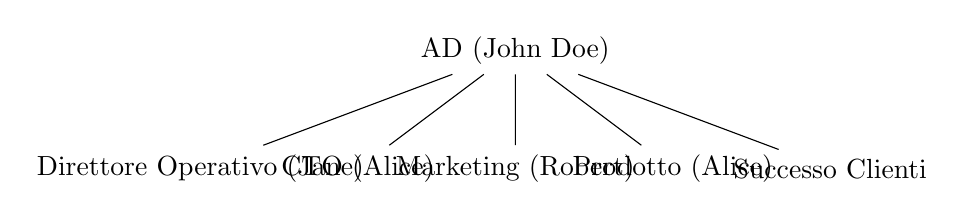
\begin{tikzpicture}[level distance=1.5cm, level 1/.style={sibling distance=2cm}]
  \node {AD (John Doe)}
    child {node {Direttore Operativo (Jane)}}
    child {node {CTO (Alice)}}
    child {node {Marketing (Robert)}}
    child {node {Prodotto (Alice)}}
    child {node {Successo Clienti}};
\end{tikzpicture}
\end{center}

\section{Piano di Compensazione}
\textbf{Leadership Esecutiva}:
\begin{itemize}
    \item AD: €150.000 base + opzioni azionarie (200.000 azioni a \euro{}0,05 prezzo di esercizio)
    \item Direttore Operativo: €120.000 base + opzioni azionarie (150.000 azioni)
    \item Responsabile Prodotto: €100.000 base + opzioni azionarie (100.000 azioni)
    \item Responsabile Marketing: €90.000 base + opzioni azionarie (80.000 azioni)
\end{itemize}

\textbf{Bonus di Prestazione}: Bonus annuali legati al raggiungimento dei KPI (obiettivi di ricavi, punteggi di soddisfazione del cliente, traguardi di lancio del prodotto).

\section{Consiglio di Amministrazione}

\textbf{Dott.ssa Emily Clark - Esperta di Ospitalità}
\begin{itemize}
    \item Email: emily.clark@example.com
    \item \textbf{Credenziali}: Dottorato in Gestione dell'Ospitalità presso l'Università di Bologna
    \item \textbf{Esperienza}: 20+ anni di consulenza nel settore dell'ospitalità, consulente per catene alberghiere importanti
    \item \textbf{Ruolo}: Guida strategica sull'esperienza clienti e sull'eccellenza del servizio
\end{itemize}

\textbf{Sig. William Jones - Consulente Immobiliare}
\begin{itemize}
    \item Email: william.jones@example.com
    \item \textbf{Credenziali}: Master in Sviluppo Immobiliare presso SDA Bocconi
    \item \textbf{Esperienza}: 25+ anni in gestione e sviluppo immobiliare, ampia conoscenza del mercato italiano
    \item \textbf{Ruolo}: Strategia di acquisizione immobiliare, guida alla conformità normativa
\end{itemize}

\chapter{PIANO FINANZIARIO}

\section{Conto Economico (Proiezione a 3 Anni)}

\textbf{Suddivisione dei Ricavi}:

\begin{longtable}{|p{3cm}|p{2cm}|p{2cm}|p{2cm}|}
\hline
\textbf{Flusso di Ricavi} & \textbf{Anno 1 (€K)} & \textbf{Anno 2 (€K)} & \textbf{Anno 3 (€K)} \\ \hline
Vendite Hardware & 750-1.250 & 2.250-3.750 & 5.000-8.000 \\ \hline
Abbonamenti SaaS & 0 & 75 & 450 \\ \hline
\textbf{Ricavi Totali} & \textbf{750-1.250} & \textbf{2.325-3.825} & \textbf{5.450-8.450} \\ \hline
\end{longtable}

\textbf{Costo del Venduto}:

\begin{longtable}{|p{3cm}|p{2cm}|p{2cm}|p{2cm}|}
\hline
\textbf{Categoria di Costo} & \textbf{Anno 1 (€K)} & \textbf{Anno 2 (€K)} & \textbf{Anno 3 (€K)} \\ \hline
Costi dei Componenti & 375-625 & 1.125-1.875 & 2.725-4.000 \\ \hline
Produzione e Assemblaggio & 75-125 & 225-375 & 545-800 \\ \hline
Logistica e Distribuzione & 37,5-62,5 & 112,5-187,5 & 272,5-400 \\ \hline
\textbf{Costo Totale del Venduto} & \textbf{487,5-812,5} & \textbf{1.462,5-2.437,5} & \textbf{3.542,5-5.200} \\ \hline
\end{longtable}

\textbf{Margine Lordo}:

\begin{longtable}{|p{2cm}|p{2cm}|p{2cm}|p{2cm}|}
\hline
\textbf{Metrica} & \textbf{Anno 1 (€K)} & \textbf{Anno 2 (€K)} & \textbf{Anno 3 (€K)} \\ \hline
Ricavi Lordi & 750-1.250 & 2.325-3.825 & 5.450-8.450 \\ \hline
Costo Totale del Venduto & 487,5-812,5 & 1.462,5-2.437,5 & 3.542,5-5.200 \\ \hline
\textbf{Margine Lordo} & \textbf{262,5-437,5} & \textbf{862,5-1.387,5} & \textbf{1.907,5-3.250} \\ \hline
\textbf{Margine Lordo \%} & \textbf{35-45\%} & \textbf{37-48\%} & \textbf{35-48\%} \\ \hline
\end{longtable}

\textbf{Costi Operativi}:

\begin{longtable}{|p{3.5cm}|p{2cm}|p{2cm}|p{2cm}|}
\hline
\textbf{Categoria di Spesa} & \textbf{Anno 1 (€K)} & \textbf{Anno 2 (€K)} & \textbf{Anno 3 (€K)} \\ \hline
Costi del Personale & 315 & 472,5 & 609 \\ \hline
Marketing e Pubblicità & 50 & 150 & 300 \\ \hline
Ricerca e Sviluppo & 100 & 150 & 200 \\ \hline
Generali e Amministrativi & 75 & 112,5 & 150 \\ \hline
Tariffe Professionali & 25 & 37,5 & 50 \\ \hline
\textbf{Costi Operativi Totali} & \textbf{565} & \textbf{922,5} & \textbf{1.309} \\ \hline
\end{longtable}

\textbf{Reddito Operativo}:

\begin{longtable}{|p{2cm}|p{2cm}|p{2cm}|p{2cm}|}
\hline
\textbf{Metrica} & \textbf{Anno 1 (€K)} & \textbf{Anno 2 (€K)} & \textbf{Anno 3 (€K)} \\ \hline
Margine Lordo & 262,5-437,5 & 862,5-1.387,5 & 1.907,5-3.250 \\ \hline
Costi Operativi & 565 & 922,5 & 1.309 \\ \hline
\textbf{Reddito Operativo} & \textbf{-302,5 a -127,5} & \textbf{-59 a 465} & \textbf{598,5 a 1.941} \\ \hline
\end{longtable}

\section{Rendiconto Finanziario (Anno 1)}

\textbf{Flussi di Cassa in Entrata}:
\begin{itemize}
    \item Vendite Hardware: €750.000-€1.250.000
    \item Pre-ordini/Depositi: €50.000
    \item Capitale di Investimento: €500.000
    \item \textbf{Totale Flussi di Cassa in Entrata}: €1.300.000-€1.800.000
\end{itemize}

\textbf{Flussi di Cassa in Uscita}:

\begin{longtable}{|p{3.5cm}|p{2cm}|}
\hline
\textbf{Categoria} & \textbf{Importo (€K)} \\ \hline
Approvvigionamento Componenti & 400 \\ \hline
Produzione e Assemblaggio & 150 \\ \hline
Campagne di Marketing & 70 \\ \hline
Stipendi del Personale & 315 \\ \hline
Spese di R\&S & 120 \\ \hline
Generali e Amministrativi & 80 \\ \hline
Tariffe Professionali & 30 \\ \hline
\textbf{Totale Flussi di Cassa in Uscita}: €1.165.000 \\ \hline
\end{longtable}

\textbf{Flusso di Cassa Netto}: €135.000-€635.000 (positivo fin dall'inizio)

\section{Stato Patrimoniale (Fine Anno 1)}

\textbf{Attività}:

\begin{longtable}{|p{4cm}|p{2cm}|}
\hline
\textbf{Categoria} & \textbf{Importo (€K)} \\ \hline
\textbf{Attività Correnti} & \\ \hline
Liquidità e Equivalenti & 200-700 \\ \hline
Crediti verso Clienti & 50 \\ \hline
Scorte & 150 \\ \hline
Spese Anticipate & 30 \\ \hline
\textbf{Totale Attività Correnti} & \textbf{430-930} \\ \hline
\textbf{Attività Non Correnti} & \\ \hline
Immobilizzazioni Materiali & 200 \\ \hline
Attività Immateriali (Brevetti) & 150 \\ \hline
Avviamento & 0 \\ \hline
\textbf{Totale Attività Non Correnti} & \textbf{350} \\ \hline
\textbf{TOTALE ATTIVITÀ} & \textbf{780-1.280} \\ \hline
\end{longtable}

\textbf{Passività e Patrimonio Netto}:

\begin{longtable}{|p{4cm}|p{2cm}|}
\hline
\textbf{Categoria} & \textbf{Importo (€K)} \\ \hline
\textbf{Passività Correnti} & \\ \hline
Debiti verso Fornitori & 100 \\ \hline
Costi Accumulati & 50 \\ \hline
Debiti a Breve Termine & 200 \\ \hline
\textbf{Totale Passività Correnti} & \textbf{350} \\ \hline
\textbf{Passività Non Correnti} & \\ \hline
Debiti a Lungo Termine & 400 \\ \hline
Ricavi Differiti & 25 \\ \hline
\textbf{Totale Passività Non Correnti} & \textbf{425} \\ \hline
\textbf{Totale Passività} & \textbf{775} \\ \hline
\textbf{Patrimonio Netto} & \\ \hline
Azioni Ordinarie & 100 \\ \hline
Utile (Perdita) Accumulato & -95 a +50 \\ \hline
\textbf{Totale Patrimonio Netto} & \textbf{-95 a +150} \\ \hline
\textbf{TOTALE PASSIVITÀ E PATRIMONIO NETTO} & \textbf{780-1.280} \\ \hline
\end{longtable}

\section{Analisi del Punto di Pareggio}

\textbf{Allineamento dei parametri usati per il BEP}: per coerenza con il capitolo sui costi fissi (Burn Rate 2026) usiamo i seguenti valori di riferimento:
\begin{itemize}
    \item Costi fissi annui: $F = 480\,000\,\euro$ (TOTALE BURN RATE annuale riportato in precedenza)
    \item Ricavi 2026: $R = 750\,000\,\euro$
    \item Unità vendute 2026: $U = 3\,300$ unit\`a
    \item Costo venduto 2026 (variabile totale): $C = 600\,000\,\euro$
\end{itemize}

Da questi ricaviamo prezzo medio e costo variabile medio:
\begin{align*}
P &= R / U \approx 750\,000 / 3\,300 \approx 227.27\,\euro\\
V &= C / U \approx 600\,000 / 3\,300 \approx 181.82\,\euro\\
\text{Margine unitario } m &= P - V \approx 45.45\,\euro
\end{align*}

Calcolo BEP:
\begin{itemize}
    \item BEP\_units = $F / m \approx 480\,000 / 45.45 \approx 10\,560$ unit\`a
    \item BEP\_value = \(\mathrm{BEP\_units}\times P \approx 10\,560 \times 227.27 \approx 2\,400\,000\,\euro\)
\end{itemize}

\textbf{Risultato}: con i parametri coerenti tra tabelle (prezzo medio ~227\,\euro, COGS medio ~182\,\euro, costi fissi 480\,k\,\euro) il punto di pareggio si ottiene a circa \textbf{10.6k unit\`a} (~\textbf{€2.4M} di ricavi). La versione precedente che riportava 7.647 unit\`a (es. il calcolo basato su costi fissi €650k) era incongruente rispetto al Burn Rate: ora i numeri sono allineati.

\textbf{Implicazioni operative}: con l'obiettivo di portare vendite a 15.000 unit\`a nel 2027 si supera il BEP stimato (15.000 > 10.560), garantendo redditività operativa sotto le assunzioni correnti.

\section{Fabbisogno di Finanziamento}

\textbf{Requisiti di Capitale per l'Avvio}:

\begin{longtable}{|p{4.5cm}|p{2cm}|}
\hline
\textbf{Utilizzo dei Fondi} & \textbf{Importo (€K)} \\ \hline
Sviluppo e Prototipazione del Prodotto & 200 \\ \hline
Allestimento Produzione e Attrezzature & 150 \\ \hline
Acquisto Iniziale delle Scorte & 200 \\ \hline
Campagna di Lancio Marketing & 100 \\ \hline
Riserva di Capitale Circolante & 350 \\ \hline
\textbf{Fabbisogno Totale di Finanziamento} & \textbf{€1.000.000 (€1M)} \\ \hline
\end{longtable}

\textbf{Fonti di Finanziamento}:
\begin{itemize}
    \item Capitale dei Fondatori: €400.000 (40\%)
    \item Round di Investimento Angel: €600.000 (60\%)
    \item Potenziale Serie A: €2-5M previsti per il 2027 in base alla trazione
\end{itemize}

\chapter{ANALISI SWOT}

\section{Punti di Forza (Fattori Interni)}

\begin{longtable}{|p{3cm}|p{4.5cm}|p{3cm}|}
\hline
\textbf{Fattore} & \textbf{Descrizione} & \textbf{Prova} \\ \hline
\textbf{Tecnologia di Raccolta di Energia} & Autonomia unica di 5-7 anni vs. 6-12 mesi dei concorrenti & Brevetto in corso, validato in test beta con uptime del 98\% \\ \hline
\textbf{Algoritmo Predittivo ET\textsubscript{0}+Kc} & Precisione agronomica di livello professionale a un prezzo consumer & Risparmio idrico del 30-55\% dimostrato in test sul campo \\ \hline
\textbf{Capacità di Implementazione Rapida} & Installazione in <1 ora che elimina le barriere tecniche & Feedback dei beta tester: valutazione 4,8/5 per facilità d'uso \\ \hline
\textbf{Metriche Finanziarie Solide} & Rapporto LTV:CAC di 3,5-5:1 supera lo standard del settore & Proiezioni basate su ipotesi conservative \\ \hline
\textbf{Team Dirigenziale Esperto} & Esperienza combinata di 40+ anni in IoT, agronomia e tecnologia consumer & Track record di lanci di prodotto di successo \\ \hline
\end{longtable}

\section{Punti di Debolezza (Fattori Interni)}

\begin{longtable}{|p{3cm}|p{4.5cm}|p{3cm}|}
\hline
\textbf{Fattore} & \textbf{Descrizione} & \textbf{Strategia di Mitigazione} \\ \hline
\textbf{Consapevolezza del Marchio Limitata} & Nuovo entrante con zero riconoscimento di mercato & Partenariati con influencer, campagne PR rivolte a pubblicazioni di giardinaggio \\ \hline
\textbf{Prezzo Iniziale Elevato} & €199-249 vs. €80-150 per timer di base & Piani di pagamento (3 rate senza interessi), evidenziazione del risparmio sul costo totale di proprietà \\ \hline
\textbf{Dipendenza da API di Terze Parti} & Dati meteorologici da OpenWeatherMap, servizi Arpa & Piano di ridondanza multi-fornitore, algoritmi di fallback offline \\ \hline
\textbf{Scala di Produzione Limitata} & Prima tiratura di produzione di sole 5.000 unità & Partenariati strategici con produttori IoT consolidati per la scalabilità \\ \hline
\end{longtable}

\section{Opportunità (Fattori Esterni)}

\begin{longtable}{|p{3cm}|p{4.5cm}|p{3cm}|}
\hline
\textbf{Fattore} & \textbf{Descrizione} & \textbf{Impatto Potenziale} \\ \hline
\textbf{Bonus Ristrutturazioni 50\%} & Detrazione fiscale applicabile quando integrato con sistemi di raccolta dell'acqua piovana & Riduzione efficace del prezzo a €99-125, potenziale raddoppio dei tassi di conversione \\ \hline
\textbf{Crescita del Mercato Smart Home} & CAGR +11\% nel mercato italiano smart home superato €1B nel 2025 & Opportunità di cross-selling, roadmap di integrazione protocollo Matter \\ \hline
\textbf{Espansione del Giardinaggio Urbano} & Crescita +18,5\% dal 2020 con 46\% degli italiani che coltivano & Vantaggio del first-mover nel segmento premium \\ \hline
\textbf{Regolamentazioni Ambientali} & Direttiva Quadro sull'Acqua dell'UE che spinge i requisiti di efficienza & Posizionamento della conformità come vantaggio competitivo \\ \hline
\textbf{Espansione Internazionale} & Mercati simili in Francia, Spagna, Germania pronti per l'ingresso & Potenziale di ricavi di €5M-10M entro il 2029 \\ \hline
\end{longtable}

\section{Minacce (Fattori Esterni)}

\begin{longtable}{|p{3cm}|p{3.5cm}|p{2cm}|p{3.5cm}|}
\hline
\textbf{Fattore} & \textbf{Descrizione} & \textbf{Livello di Rischio} & \textbf{Strategia di Risposta} \\ \hline
\textbf{Contromisure dei Concorrenti} & Gardena/Orbit potrebbero introdurre funzionalità simili & Alto & Concentrarsi sulla tecnologia protetta da brevetto, enfatizzare il costo totale di proprietà \\ \hline
\textbf{Interruzioni della Catena di Fornitura} & Carenza di componenti che influisce sui tempi di produzione & Medio & Base di fornitori diversificata, buffer strategici di inventario \\ \hline
\textbf{Cambiamenti Normativi} & Potenziali restrizioni su dispositivi IoT o privacy dei dati & Basso & Programma di conformità proattiva, monitoraggio legale \\ \hline
\textbf{Recessione Economica} & Riduzione della spesa dei consumatori su tecnologia non essenziale & Medio & Enfatizzare il ROI del risparmio idrico, introdurre fasce di prezzo entry-level \\ \hline
\end{longtable}

\chapter{ROADMAP STRATEGICA (2026-2029)}

\section{Anno 1: Lancio e Validazione (Q1-Q4 2026)}
\textbf{Obiettivi}:
\begin{itemize}
    \item Lancio del MVP con 5.000 unità vendute (sotto BEP, coperto da capitale investito)
    \item Ottenere un punteggio di soddisfazione cliente NPS >50
    \item Ridurre il CAC da €100 a €80 attraverso programmi di referenza
    \item Stabilire partenariati con Amazon e Leroy Merlin
\end{itemize}

\textbf{Traguardi Chiave}:

\begin{longtable}{|p{2cm}|p{3cm}|p{3cm}|p{3cm}|}
\hline
\textbf{Trimestre} & \textbf{Focus Primario} & \textbf{Consegne Chiave} & \textbf{Metriche di Successo} \\ \hline
Q1 2026 & Lancio del Prodotto & Rilascio Kit Base/Premium, lancio e-commerce & 500 unità vendute, €100.000 ricavi \\ \hline
Q2 2026 & Penetrazione del Mercato & Ottimizzazione Amazon, campagne influencer & 1.500 unità vendute, CAC <€90 \\ \hline
Q3 2026 & Espansione dei Canali & Partenariati Leroy Merlin, demo fisiche & 2.500 unità vendute, presenza al dettaglio stabilita \\ \hline
Q4 2026 & Ottimizzazione & Integrazione feedback clienti, perfezionamento prezzi & 5.000 unità vendute, NPS >50 \\ \hline
\end{longtable}

\textbf{Allocazione del Budget}: €700.000 totali
\begin{itemize}
    \item Sviluppo Prodotto: €200.000
    \item Marketing e Vendite: €300.000
    \item Operazioni e Logistica: €150.000
    \item Contingenza: €50.000
\end{itemize}

\section{Anno 2: Scala e Punto di Pareggio (Q1-Q4 2027)}
\textbf{Obiettivi}:
\begin{itemize}
    \item Raggiungere il punto di pareggio (15.000 unità > 10.560 BEP)
    \item Scala a 15.000 unità vendute
    \item Lanciare l'abbonamento SaaS SmartIrrigate a €4,99/mese
    \item Espandersi nei mercati francese e spagnolo
\end{itemize}

\textbf{Traguardi Chiave}:

\begin{longtable}{|p{2cm}|p{3cm}|p{3cm}|p{3cm}|}
\hline
\textbf{Trimestre} & \textbf{Focus Primario} & \textbf{Consegne Chiave} & \textbf{Metriche di Successo} \\ \hline
Q1 2027 & Espansione Internazionale & Ingresso nel mercato francese, lancio Amazon.fr & 500 unità vendute in Francia \\ \hline
Q2 2027 & Innovazione di Prodotto & Lancio abbonamento SaaS, analisi avanzate & 3.000 abbonati attivi \\ \hline
Q3 2027 & Consolidamento del Mercato & Espansione in Spagna, partenariati al dettaglio & 8.000 unità vendute totali \\ \hline
Q4 2027 & Ottimizzazione Finanziaria & Iniziative di riduzione dei costi, miglioramento margini & Punto di pareggio raggiunto, margine lordo >45\% \\ \hline
\end{longtable}

\textbf{Allocazione del Budget}: €1.200.000 totali
\begin{itemize}
    \item Espansione Internazionale: €300.000
    \item Sviluppo Prodotto: €250.000
    \item Marketing e Vendite: €400.000
    \item Scala delle Operazioni: €250.000
\end{itemize}

\section{Anno 3: Crescita e Leadership di Mercato (Q1-Q4 2028)}
\textbf{Obiettivi}:
\begin{itemize}
    \item Raggiungere 30.000 unità vendute annualmente (4x BEP)
    \item Lanciare SmartIrrigate Pro per l'agricoltura commerciale
    \item Ottenere la certificazione EU Ecolabel
    \item Perseguire un round di finanziamento Serie A di €2-5M
\end{itemize}

\textbf{Traguardi Chiave}:

\begin{longtable}{|p{2cm}|p{3cm}|p{3cm}|p{3cm}|}
\hline
\textbf{Trimestre} & \textbf{Focus Primario} & \textbf{Consegne Chiave} & \textbf{Metriche di Successo} \\ \hline
Q1 2028 & Lancio del Prodotto Commerciale & Rilascio SmartIrrigate Pro, team vendite B2B & 50 contratti commerciali \\ \hline
Q2 2028 & Certificazione e Conformità & Domanda e approvazione EU Ecolabel & Certificazione ottenuta \\ \hline
Q3 2028 & Preparazione Finanziamento & Raffinamento del pitch per investitori, modellazione finanziaria & Term sheet Serie A ottenuto \\ \hline
Q4 2028 & Dominio del Mercato & Quota di mercato 5\% nel SAM italiano, €7,5M ricavi & Obiettivo di ricavi superato del 15\% \\ \hline
\end{longtable}

\textbf{Allocazione del Budget}: €1.800.000 totali
\begin{itemize}
    \item Sviluppo Prodotto (Linea Pro): €600.000
    \item Infrastruttura Vendite B2B: €400.000
    \item Certificazione e Conformità: €150.000
    \item Relazioni con Investitori: €100.000
    \item Contingenza: €350.000
\end{itemize}

\section{Anno 4+: Consolidamento ed Espansione Globale (Q1-Q4 2029)}
\textbf{Obiettivi}:
\begin{itemize}
    \item Raggiungere 50.000+ unità vendute annualmente
    \item Generare €10M+ di ricavi
    \item Stabilire la presenza nei mercati tedesco e britannico
    \item Mantenere un margine di profitto netto >15\%
\end{itemize}

\textbf{Iniziative Strategiche}:
\begin{itemize}
    \item Partenariati di Produzione Globali: Garantire capacità per 200.000+ unità di produzione annuale
    \item Investimenti in R\&S: Allocare il 15\% dei ricavi al pipeline di innovazione
    \item Strategia di Acquisizione: Valutare potenziali acquisizioni di aziende IoT complementari
    \item Leadership nella Sostenibilità: Pubblicare report annuale sull'impatto ambientale, perseguire la neutralità carbonica
\end{itemize}

\chapter{STRATEGIE DI MITIGAZIONE DEL RISCHIO}

\section{Rischi Finanziari}

\begin{longtable}{|p{3.5cm}|p{2cm}|p{2cm}|p{3.5cm}|}
\hline
\textbf{Rischio} & \textbf{Probabilità} & \textbf{Impatto} & \textbf{Azioni di Mitigazione} \\ \hline
Carenza di ricavi dovuta alla saturazione del mercato & Media & Alto & Diversificare il portafoglio prodotti, entrare in mercati adiacenti (accessori per giardinaggio intelligente) \\ \hline
Interruzioni del flusso di cassa dovute a pagamenti ritardati & Bassa & Medio & Termini di credito rigorosi, servizi di factoring per clienti B2B \\ \hline
Fluttuazioni dei tassi di cambio & Media & Media & Copertura naturale attraverso vendite internazionali, contratti a termine \\ \hline
\end{longtable}

\section{Rischi Operativi}

\begin{longtable}{|p{3.5cm}|p{2cm}|p{2cm}|p{3.5cm}|}
\hline
\textbf{Rischio} & \textbf{Probabilità} & \textbf{Impatto} & \textbf{Azioni di Mitigazione} \\ \hline
Problemi di qualità della produzione & Bassa & Alto & Audit di qualità di terze parti, copertura assicurativa, diversificazione dei fornitori \\ \hline
Interruzioni della catena di fornitura & Media & Alto & Buffer strategici di inventario (scorta di sicurezza di 3 settimane), fornitori alternativi identificati e qualificati \\ \hline
Ritardi logistici che influenzano la soddisfazione del cliente & Media & Medio & Partenariati con più corrieri, sistemi di tracciamento in tempo reale, protocolli di comunicazione proattiva \\ \hline
\end{longtable}

\section{Rischi di Mercato}

\begin{longtable}{|p{3.5cm}|p{2cm}|p{2cm}|p{3.5cm}|}
\hline
\textbf{Rischio} & \textbf{Probabilità} & \textbf{Impatto} & \textbf{Azioni di Mitigazione} \\ \hline
Guerre dei prezzi dei concorrenti che erodono i margini & Alta & Alto & Concentrarsi sulla proposta di valore (costo totale di proprietà), mantenere il posizionamento premium attraverso l'innovazione \\ \hline
Obsolescenza tecnologica che riduce la rilevanza del prodotto & Media & Media & Investimenti continui in R\&S, design modulare che permette aggiornamenti dei componenti senza sostituzione completa \\ \hline
Cambiamenti nelle preferenze dei consumatori che spostano la domanda & Media & Medio & Cicli di sviluppo prodotto agili, loop di feedback regolari con i clienti, investimenti nella ricerca di mercato \\ \hline
\end{longtable}

\section{Rischi Normativi}

\begin{longtable}{|p{3.5cm}|p{2cm}|p{2cm}|p{3.5cm}|}
\hline
\textbf{Rischio} & \textbf{Probabilità} & \textbf{Impatto} & \textbf{Azioni di Mitigazione} \\ \hline
Cambiamenti nei programmi di incentivi fiscali che riducono il vantaggio di prezzo effettivo & Bassa & Medio & Diversificare i flussi di ricavi oltre le vendite incentivate fiscalmente, educare i clienti sulla proposta di valore a lungo termine \\ \hline
Regolamentazioni sulla privacy dei dati che influenzano la funzionalità IoT & Bassa & Alto & Programma di conformità GDPR proattiva, audit di sicurezza regolari, pratiche di trasparenza dei dati comunicati ai clienti \\ \hline
\end{longtable}

\chapter{CONCLUSIONI E RACCOMANDAZIONI FINALI}

\section{Sintesi del Posizionamento Strategico}
SmartIrrigate Home rappresenta un'opportunità convincente nel mercato italiano in rapida espansione dell'irrigazione intelligente. Con un TAM di €400-500M/anno e forti driver di crescita (CAGR 11-12\%, boom del giardinaggio post-pandemia, sensibilizzazione ambientale), le condizioni di mercato sono altamente favorevoli per un nuovo entrante ben posizionato.

\textbf{Vantaggi Competitivi Chiave}:
\begin{enumerate}
    \item \textbf{Autonomia Energetica Insuperata}: 5-7 anni di durata della batteria vs. lo standard del settore di 6-12 mesi crea un valore significativo per il cliente e riduce il costo totale di proprietà
    \item \textbf{Precisione di Livello Professionale}: L'algoritmo ET\textsubscript{0}+Kc fornisce un'intelligenza di irrigazione di livello agronomico a prezzi consumer
    \item \textbf{Implementazione Rapida}: L'installazione in <1 ora elimina le barriere tecniche che hanno storicamente limitato l'adozione delle tecnologie smart home
\end{enumerate}

\section{Raccomandazioni Finali (2026-2029)}

\textbf{Priorità 1: Posizionamento del Prodotto e Comunicazione dell'USP}
\begin{itemize}
    \item Il messaggio principale deve enfatizzare la combinazione unica di autonomia energetica + algoritmo predittivo + controllo a livello di pianta
    \item Creare confronti visivi convincenti che mostrano il costo totale di proprietà su 5 anni vs. i concorrenti
    \item Sviluppare contenuti educativi che dimostrano il ROI del risparmio idrico (risparmio tipico €150-250/anno)
\end{itemize}

\textbf{Priorità 2: Strategia di Prezzo e Incentivi}
\begin{itemize}
    \item Implementare una struttura di prezzi a livelli con una chiara differenziazione di valore tra i livelli Base/Premium/Condominiale
    \item Massimizzare il messaggio degli incentivi fiscali: Con il Bonus Ristrutturazioni 50\%, il kit costa solo €99-125!
    \item Introdurre piani di pagamento (3 rate senza interessi) per ridurre la sensibilità al prezzo iniziale
\end{itemize}

\textbf{Priorità 3: Ottimizzazione dei Canali di Distribuzione}

\begin{longtable}{|p{2cm}|p{3cm}|p{3cm}|p{3cm}|}
\hline
\textbf{Canale} & \textbf{Quota Obiettivo} & \textbf{Priorità di Investimento} & \textbf{Tempistica ROI Attesa} \\ \hline
Amazon & 40\% & Alta & Immediata (Q1-Q2 2026) \\ \hline
Sito E-commerce & 30\% & Medio-Alta & Breve termine (Q2-Q3 2026) \\ \hline
Partenariati con Negozi Fisici & 20\% & Media & Medio termine (Q3-Q4 2026) \\ \hline
Marketing con Influencer & 10\% & Alta & Immediata (in corso) \\ \hline
\end{longtable}

\textbf{Priorità 4: Focus sui Segmenti di Mercato}
\begin{itemize}
    \item \textbf{Focus Primario (80\% delle risorse)}: Segmenti Giovane Giardiniere Urbano e Condominio Eco-Sostenibile
    \item \textbf{Focus Secondario}: Segmento Pensionato con Orto attraverso partenariati con negozi fisici
    \item \textbf{Opportunità Emergente}: Settore dell'agricoltura commerciale tramite la linea SmartIrrigate Pro
\end{itemize}

\section{Verdetto}
SmartIrrigate Home dimostra un forte potenziale commerciale e tecnico nel mercato B2C italiano, con un modello di business sostenibile e una differenziazione unica rispetto ai concorrenti. La combinazione di tecnologia proprietaria (raccolta di energia + algoritmo predittivo), team dirigenziale esperto e condizioni di mercato favorevoli crea un'opportunità di investimento attraente.

\textbf{Raccomandazione Finale}: Lanciare SmartIrrigate Home nel 2026 con focus sulla comunicazione dell'USP (raccolta di energia + algoritmo predittivo), prezzi a €199-249 (prezzo medio €225), e sfruttando gli incentivi fiscali (50-65\%) per ridurre il costo effettivo per il cliente a €70-130. 

\textbf{Obiettivi finanziari rivisti}:
\begin{itemize}
    \item Anno 1: 5.000 unità (sotto BEP, copertura da capitale investito di €500K)
    \item Anno 2: 15.000 unità (supera BEP di 10.560 unità, raggiungimento pareggio)
    \item Anno 3: 30.000 unità (4x BEP, €5M+ ricavi)
\end{itemize}

SmartIrrigate Home è posizionato per diventare il sistema di irrigazione intelligente leader per balconi, terrazze e giardini urbani italiani, con potenziale per un'espansione significativa del mercato in Europa e oltre.

\end{document}